% --------------------------------------------------------------
% This is all preamble stuff that you don't have to worry about.
% Head down to where it says "Start here"
% --------------------------------------------------------------
 
\documentclass[12pt]{article}
 
\usepackage[margin=1in]{geometry} 
\usepackage{amsmath,amsthm,amssymb}
\usepackage{graphicx}

\begin{document}
 
% --------------------------------------------------------------
%                         Start here
% --------------------------------------------------------------
 
\title{Practical No. 2 }%replace X with the appropriate number
\author{Maciej Domaradzki\\ %replace with your name
md406127@students.mimuw.edu.pl}
 
\maketitle
 
\section{Part 1 }
\subsection*{a) }

\[
-\sum_{w \in \text{Vocab}} y_w \log{\hat{y}_w} = 
- (\sum_{w \in \text{Vocab}, y_w \neq y_o} y_w \log{\hat{y}_w} + y_o \log{\hat{y}_o})
\]
\[
- (\sum_{w \in \text{Vocab}, y_w \neq y_o} 0 \cdot \log{\hat{y}_w} + 1 \cdot \log{\hat{y}_o)
= - \log{\hat{y}_o}}
\]

\subsection*{b) }

\[
\frac{\partial J_{\text{Naive-Softmax}}}{\partial v_c} (v_c, o, U)
= - \frac{\partial}{\partial v_c} \log{\frac{ \exp (u_o^T v_c)}{\sum_{w \in \text{Vocab}}  \exp (u_w^T v_c)}}
= - \frac{\partial}{\partial v_c} (u_o^T v_c - \log{\sum_{w \in \text{Vocab}}  \exp (u_w^T v_c)})
\]
\[
= - (u_o  - \frac{\sum_{w \in \text{Vocab}} \exp (u_w^T v_c)  u_w}{\sum_{w \in \text{Vocab}}  \exp (u_w^T v_c)})
= - (u_o  - \sum_{w \in \text{Vocab}} P(O=w|C=c) u_w)
= - (u_o  - \sum_{w \in \text{Vocab}} \hat{y}_w u_w)
\]
\[
= - u_o + \sum_{w \in \text{Vocab}} \hat{y}_w u_w
= U(\hat{y} - y)
\]

\subsection*{c) }

\[
\frac{\partial J_{\text{Naive-Softmax}}}{\partial u_w} (v_c, o, U)
= - \frac{\partial}{\partial u_w} \log{\frac{ \exp (u_o^T v_c)}{\sum_{w \in \text{Vocab}}  \exp (u_w^T v_c)}}
= - \frac{\partial}{\partial u_w} (u_o^T v_c - \log{\sum_{w \in \text{Vocab}}  \exp (u_w^T v_c)})
\]
\[
= - (\frac{\partial}{\partial u_w}  u_o^T v_c - \frac{\partial}{\partial u_w} \log{\sum_{w \in \text{Vocab}}  \exp (u_w^T v_c)})
\]

If $w \neq o$:

\[
\frac{\partial J_{\text{Naive-Softmax}}}{\partial u_w} (v_c, o, U)
= - (0 -  \frac{\exp (u_w^T v_c)  v_c}{\sum_{w \in \text{Vocab}}  \exp (u_w^T v_c)})
= - (0 - P(O=w|C=c) v_c)
\]
\[
= P(O=w|C=c) v_c
= \hat{y}_w v_c
\]

If $w = o$:

\[
\frac{\partial J_{\text{Naive-Softmax}}}{\partial u_w} (v_c, o, U)
= - (v_c -  \frac{\exp (u_w^T v_c)  v_c}{\sum_{w \in \text{Vocab}}  \exp (u_w^T v_c)})
= - (v_c - P(O=w|C=c) v_c)
\]
\[
= (P(O=w|C=c) - 1) v_c
= (\hat{y}_w - 1) v_c
\]

\subsection*{d) }

\[
\frac{\partial \sigma(x)}{\partial x} = [\frac{\partial \sigma(x_i)}{\partial x_j}]_{N \times N}
\]
\[
= \begin{bmatrix}
\frac{\partial \sigma(x_1)}{\partial x_1} & 0 & \vdots & 0\\
0 & \frac{\partial \sigma(x_2)}{\partial x_2} & \vdots & 0\\
\ldots & \ldots & \ldots & \ldots\\
0 & 0 & \vdots & \frac{\partial \sigma(x_n)}{\partial x_n}
\end{bmatrix}
\]

\[
\frac{\partial \sigma(x_i)}{\partial x_i} = \sigma(x_i) (1-\sigma(x_i))
\]

\subsection*{e) }

\[
\frac{\partial J_{\text{neg-sample}}}{\partial v_c} (v_c, o, U) 
= (\sigma(u_o^T v_c) - 1) u_o + \sum_{k=1}^K (1-\sigma(-u_k^T v_c)) u_k
\]
\[
= (\sigma(u_o^T v_c) - 1) u_o + \sum_{k=1}^K (\sigma(u_k^T v_c)) u_k
\]

\[
\frac{\partial J_{\text{neg-sample}}}{\partial u_o} (v_c, o, U) 
= (\sigma(u_o^T v_c) - 1) v_c
\]

\[
\frac{\partial J_{\text{neg-sample}}}{\partial u_k} (v_c, o, U) 
= (\sigma(u_k^T v_c)) v_c
\]

\subsection*{f) }

\[
\frac{\partial J_{\text{skip-gram}}}{\partial U} (v_c, w_{t-m}, \ldots, w_{t+m}, U) 
\sum_{-m \leq m, j \neq 0} \frac{\partial J_{\text{neg-sample}}}{\partial U} (v_c, w_{t+i}, U)
\]

\[
\frac{\partial J_{\text{skip-gram}}}{\partial v_c} (v_c, w_{t-m}, \ldots, w_{t+m}, U)
\sum_{-m \leq m, j \neq 0} \frac{\partial J_{\text{neg-sample}}}{\partial v_c} (v_c, w_{t+i}, U) 
\]

\[
\frac{\partial J_{\text{skip-gram}}}{\partial v_w} (v_c, w_{t-m}, \ldots, w_{t+m}, U)
= 0
\]

\section{Part 2 }

\begin{figure}[!h]
\centering
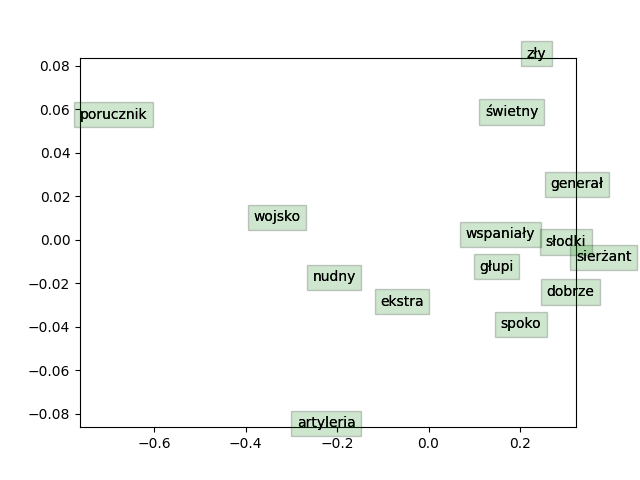
\includegraphics{word_vectors.png}
\caption{\text{word vectors}}
\label{fig:image}
\end{figure}

In the picture we can see that adverbs "dobrze" and "spoko" are close to each other. Words "sierżant" and "generał" are close to each other, but "porucznik" is far from those two. Adjectives having opposite meaning are also close to each other, for example "głupi" and "wspaniały" or "zły" i "świetny".

\section{Part 3 }
\subsection*{a) }

Using $m$ causes update to be only a little influenced by current gradient and mostly influenced by its history of change, so sudden change of gradient doesn't cause in sudden change of update, so updates are more stable. Thanks to it  the changes are smoother and we can use bigger learning rates. 

\subsection*{b) }
It scales up changes for parameters, which gradients are small and scales down for those, which gradients are big. It help us in situations, when gradient is big in some direction, but small in other.
 
\subsection*{d) }
Dropout helps our net to generalize better. Thanks to this more neurons are responsible for similar tasks and thanks to this are network is more robust during evaluation.

% --------------------------------------------------------------
%     You don't have to mess with anything below this line.
% --------------------------------------------------------------
 
\end{document}